\begin{figure}[!htbp]
\centering
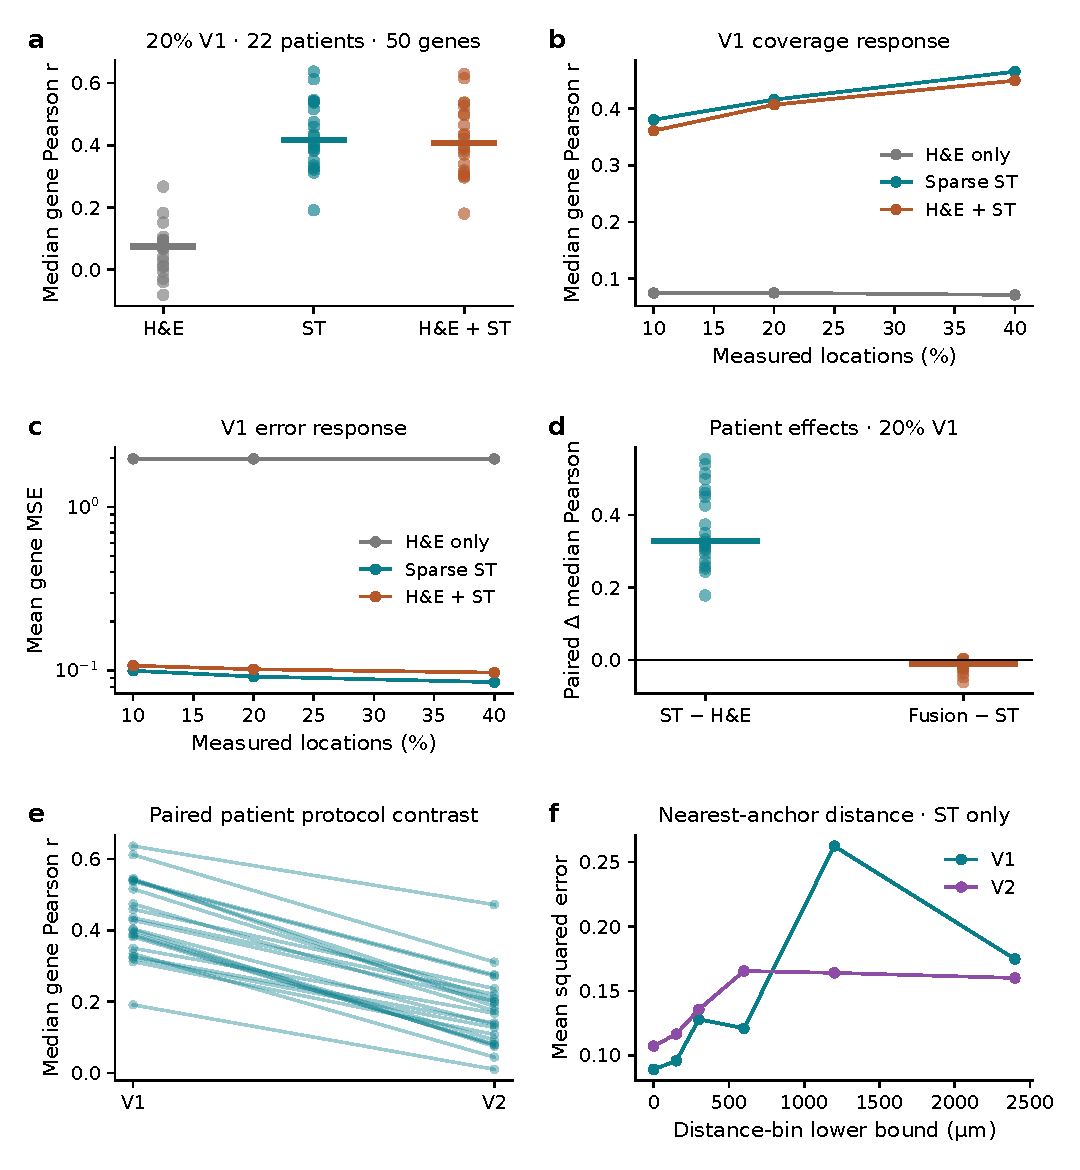
\includegraphics[width=\textwidth,height=0.70\textheight,keepaspectratio]{figures/Figure5.pdf}
\caption{\textbf{Independent 22-patient replication confirms the coverage response and weaker contiguous completion.} One first-numbered section per Bassiouni patient was selected before evaluation, yielding 30,003 locations and the same 50 primary genes. No patient from this study was used for new training or calibration. \textbf{a,} Patient correlation summaries at 20\% distributed coverage. \textbf{b,c,} Correlation and MSE across measurement fractions. \textbf{d,} Paired interpolation--image and fusion--interpolation correlation effects. \textbf{e,} Paired V1/V2 molecular correlations at 20\%. \textbf{f,} Distance-resolved molecular MSE at 20\%. Each patient summary averages ten mask seeds within geometry and then the three V2 geometry means where applicable; cohort curves use patient medians. All 22 patients improved in correlation and MSE between 10\% and 40\% V1 coverage and deteriorated in correlation, MSE and MAE under V2 relative to V1 at 20\%. V1/V2 differ in scoring support and interpolation weighting as well as missing-region design. Image fusion uses the frozen Wu calibration and 0.2 image weight. Public histology contained only 24--29 native pixels per 112-\um{} patch. Distance curves have varying occupied-bin support and are not calibrated uncertainty intervals. No p-values or patient confidence intervals are implied.}
\label{fig:bassiouni}
\end{figure}
